\documentclass[11pt]{article}
\usepackage{geometry}           
\geometry{letterpaper}                   

\usepackage{graphicx}
\usepackage{amssymb}
\usepackage{epstopdf}
\usepackage{natbib}
\usepackage{amssymb, amsmath}
\usepackage{listings}
\usepackage{inconsolata}
\usepackage{xcolor}
\usepackage[nottoc,numbib]{tocbibind}
\usepackage{float}

\definecolor{codeRed}{RGB}{231,76,60}
\definecolor{codeBlue}{RGB}{52,152,219}
\definecolor{codePurple}{RGB}{155,89,182}
\definecolor{codeDarkBlue}{RGB}{52,73,94}

\lstdefinelanguage{JavaScript}{
  keywords={typeof, new, catch, function, null, catch, switch, if, in, while, do, else, case, break, for, return, continue},
  keywordstyle=\color{codeBlue}\bfseries,
  ndkeywords={class, export, boolean, throw, implements, import, this, var, let, const, int, double, char, true, false},
  ndkeywordstyle=\color{codePurple}\bfseries,
  identifierstyle=\color{codeBlue},
  sensitive=false,
  comment=[l]{//},
  morecomment=[s]{/*}{*/},
  commentstyle=\color{gray}\ttfamily,
  stringstyle=\color{codeRed}\ttfamily,
  morestring=[b]',
  morestring=[b]"
}

\lstset{
   language=JavaScript,
   backgroundcolor=\color{white},
   extendedchars=true,
   basicstyle=\footnotesize\ttfamily,
   showstringspaces=false,
   showspaces=false,
   numbers=left,
   numberstyle=\footnotesize,
   numbersep=9pt,
   tabsize=2,
   breaklines=true,
   showtabs=false,
   captionpos=b
}

\DeclareGraphicsRule{.tif}{png}{.png}{`convert #1 `dirname #1`/`basename #1 .tif`.png}

\title{Burning Man}
\author{Nico Hauser, Andri Horat, Elias Schmid, Jonas Spieler}
\date{date}

\begin{document}



\thispagestyle{empty}

\begin{center}
\includegraphics[width=5cm]{ETHlogo.eps}

\bigskip


\bigskip


\bigskip


\LARGE{ Burning Man:\\ }
\LARGE{ Simulating the behaviour of people in the event of fire\\}

\bigskip

\bigskip

\small{Project Report}\\

\bigskip

\bigskip

\bigskip

\bigskip


% \begin{tabular}{|c|}
% \hline
% \\
% \textbf{\LARGE{Burning Man}}\\
% \\
% \hline
% \end{tabular}
\bigskip

\bigskip

\bigskip

\LARGE{Nico Hauser, Andri Horat, Elias Schmid, Jonas Spieler}



\bigskip

\bigskip

\bigskip

\bigskip

\bigskip

\bigskip

\bigskip

\bigskip

Zurich\\
May 2008\\

\end{center}



\newpage

%%%%%%%%%%%%%%%%%%%%%%%%%%%%%%%%%%%%%%%%%%%%%%%%%

\newpage
\section*{Agreement for free-download}
\bigskip


\bigskip


\large We hereby agree to make our source code for this project freely available for download from the web pages of the SOMS chair. Furthermore, we assure that all source code is written by ourselves and is not violating any copyright restrictions.

\begin{center}

\bigskip


\bigskip


\begin{tabular}{@{}p{3.3cm}@{}p{6cm}@{}@{}p{6cm}@{}}
\begin{minipage}{3cm}

\end{minipage}
&
\begin{minipage}{6cm}
\vspace{2mm} \large Nico Hauser
 \vspace{\baselineskip}

\end{minipage}
&
\begin{minipage}{6cm}

\large Andri Horat

\end{minipage}
\\
\\
\\
\\
\\
\begin{minipage}{3cm}

\end{minipage}
&
\begin{minipage}{6cm}
\vspace{2mm} \large Elias Schmid

 \vspace{\baselineskip}

\end{minipage}
&
\begin{minipage}{6cm}

\large Jonas Spieler

\end{minipage}
\end{tabular}


\end{center}
\newpage

%%%%%%%%%%%%%%%%%%%%%%%%%%%%%%%%%%%%%%%



% IMPORTANT
% you MUST include the ETH declaration of originality here; it is available for download on the course website or at http://www.ethz.ch/faculty/exams/plagiarism/index_EN; it can be printed as pdf and should be filled out in handwriting


%%%%%%%%%% Table of content %%%%%%%%%%%%%%%%%

\tableofcontents

\newpage

%%%%%%%%%%%%%%%%%%%%%%%%%%%%%%%%%%%%%%%



\section{Abstract}

This paper describes a model for the behaviour of people in the event of fire and it's simulation. The model tries to incorporate the general repulsion of people standing too close, the formation of groups in panic situations, the placement of exit signs and many other factors such as different speeds. In order to make observations on the defined model, it is simulated using a physics engine using javascript that makes it accessible from any place at any time and allows for reproducible and verifiable results. The paper defines a general parameterized model of the environment and the agents which, with the right choice of simulation parameters, even allow for a safety evaluation of specific settings. Simulations using this model were able to verify results of other papers but also put them into perspective.

\section{Introduction and Motivations}

This paper was created during the course \textit{Agent-Based Modeling and Social System Simulation} held by Dr. Nino Antulov-Fantulin and Thomas Asikis at ETH Zurich. The goal was to create a project matching the title of the course meaning the modelling of a complex system where humans are the agents. A complex system is in contrast to complicated system not per se hard to implement but rather consists of many simple small parts that on themselves act based on simple rules. The fact that there are a lot of these so-called agents gives rise to behaviours of the whole system that are not always easy to predict or even understand even if the simple rules of a single agent are well-known. As computers keep getting faster and new technology is developed every day, simulations are a good way of understanding these complex systems by playing with the available parameters while looking for emerging patterns and applying them to the real world.

\section{Description of the Model}

For readability this chapter is split as the definition of the environment is to some extent independent of the agent's model.

\subsection{Environment model}

Before agents can react to a fire an environment has to be created which in our case is a building. As the environment is one of the parameters that in a successful model should be easy to change, a subset of a preexisting format definition is used. The environment consists of the so-called object layers \texttt{signs}, \texttt{agents}, \texttt{doors}, \texttt{physical-walls}, \texttt{navmesh} and \texttt{despawn-zones}. The \texttt{signs} and \texttt{doors} layers contain points indicating the position of the safety signs and the doors. They are separate as they represent different things. The safety signs represent actual signs that the agents follow should they be visible. The location of the doors on the other hand are remembered by the agents and thus do not have to be visible for the agent to know it's location. In addition both signs can have the two properties \texttt{orientationX} and \texttt{orientationY} indicating the direction of a $180$ degree angle from which the sign is visible. Another property signs can have is \texttt{radius} which, if defined, overrides the default radius for marking a sign as visited. The reasons will be made clear in the description of the agent model. The \texttt{agents} layer also consists of points indicating the spawn points of the agents. \texttt{physical-walls}, as the name might suggest, defines the location of the walls using rectangles. This layer is used for giving the environment a shape as the agents cannot walk through these walls. In addition this layer is used for the raytracing algorithm as the agents should not be able to see signs if there's a wall in between but more to that in the agent model description. The \texttt{navmesh} layer defines the navigation mesh mode of rectangles. This mesh defines the points an agent can use for navigation when walking into the direction of a sign or a door. The details of this navigation mesh are also described in the next section about the agent model. Last but not least there's the \texttt{despawn-zones} layer where rectangles are used to define areas that will, when colliding with an agent, remove it from the simulation and count them as in safety.

\subsection{Agent model}
For the agent model a so-called social force model is used. In short agents behave like particles in newtonian physics. Every agent has a mass, position and velocity and on every agent act a bunch of forces resulting in an acceleration according to the famous $F=m\cdot a$. The agents representing the people are approximated as a circle in the physics engine where each agent has different intrinsic properties, most of which are generated randomly based on a normal distribution with selected mean and standard deviation values. To have more realistic values we cap the random distribution within the standard deviation as the actual probability of some value far away would otherwise not be zero, just very small.

First we calculate the basic properties \texttt{weight, fitness} and \texttt{age} based on the described capped normal distribution. The radius or size of the agent is then also chosen from the capped normal distrubution but is then also multiplied with the \textit{normalized} \texttt{weight} and divided by the \textit{normalized} \texttt{fitness}. By \textit{normalized} we refer to the proportion of the random value to the mean for the given value. This factor $\frac{1}{\texttt{|agility|}} = \frac{\texttt{|weight|}}{\texttt{|fitness|}}$ (the $|\cdot|$ refers to the \textit{normalized} value) or rather its inverse is also used when generating the \texttt{maxVelocity} and the \texttt{maxAcceleration}, both of these values are multipled with this factor \texttt{agility} after being randomly chosen from the respective capped normal distrubution. As visual sight is a very important in emergency situations for finding safety signs and can also be disturbed by for example smoke, the property \texttt{visualRange} is also generated from another capped normal distribution whose result is then divided by the \textit{normalized} age.

After the generation of these random values, the agents are a sole product of their environment and their behaviour is based on a set of simple rules.

\begin{itemize}
    \item Wall repulsion
    
    To model human behaviour, agents should in general prefer to move away from walls as most humans prefer to have some space around them.

    \item Agent repulsion
    
    For the same reason people do not like to stand close to each other, especially not in emergency situations. To model this, the agents will thus move away from each other if their distance is small.

    \item Agent attraction
    
    Even tough people do not like to stand close to each other, they still tend to form groups and do not like to act on their own. Thus the agents are instructed to move closer together as long as the distance between them is in the acceptable range.

    \item Target attraction
    
    Last but definitely not least, the agents have to do something and not just stand around. In the best case, the agents should try to reach one of the defined escape zones. In real life, safety signs guide people to these safe zones so the agents are instructed to always be on the lookout for visible signs guiding them to safety. In real life not all small rooms do have safety signs in them as for humans the only viable option in an emergency is to first leave the room they're in. As the agents should follow this behaviour, doors function similar to signs except that they do not have to be visible. This allows to simulate some kind of memory of the agents and enables them to leave the room even without have seen a safety sign. Another type of memory that is simulated is the remembrance of already visited signs and doors as real humans will not follow the same sign twice if the direction the sign points in didn't lead to an exit the first time around. An exception is made to this, when an agent doesn't have any target anymore they ''forget'' everything they visited before and start from scratch. This allows for some more complex behaviours such as an agent being pushed back into the room he just was in because of other agents rushing the hallway. If the memory wasn't cleared, the agent now wouldn't leave the room a second time which of course would be a real bad behaviour.
\end{itemize}

\section{Implementation}

The implementation of this model is done in javascript using a game library called phaser that already includes a physics engine and has means of drawing the result onto a \texttt{HTML} canvas meaning the whole simulation can easily be rendered on a webpage and doesn't require any setup.

\subsection{Environment construction}
As people are at least to some extent the product of their environment, it is very important that the simulations does not have a fixed environment in which all simulations take place. In fact it is one of the most important parameters when looking at the results, i.e. how many people survived a fire emergency. People in a totally enclosed room have no chance of escaping whereas agents sitting next to an escape zone will have no issues. To make the change of this parameter as accessible as possible, the implementation uses an open source format called \texttt{Tiled's map format} (TMX).

\begin{figure}[H]
	\centering
	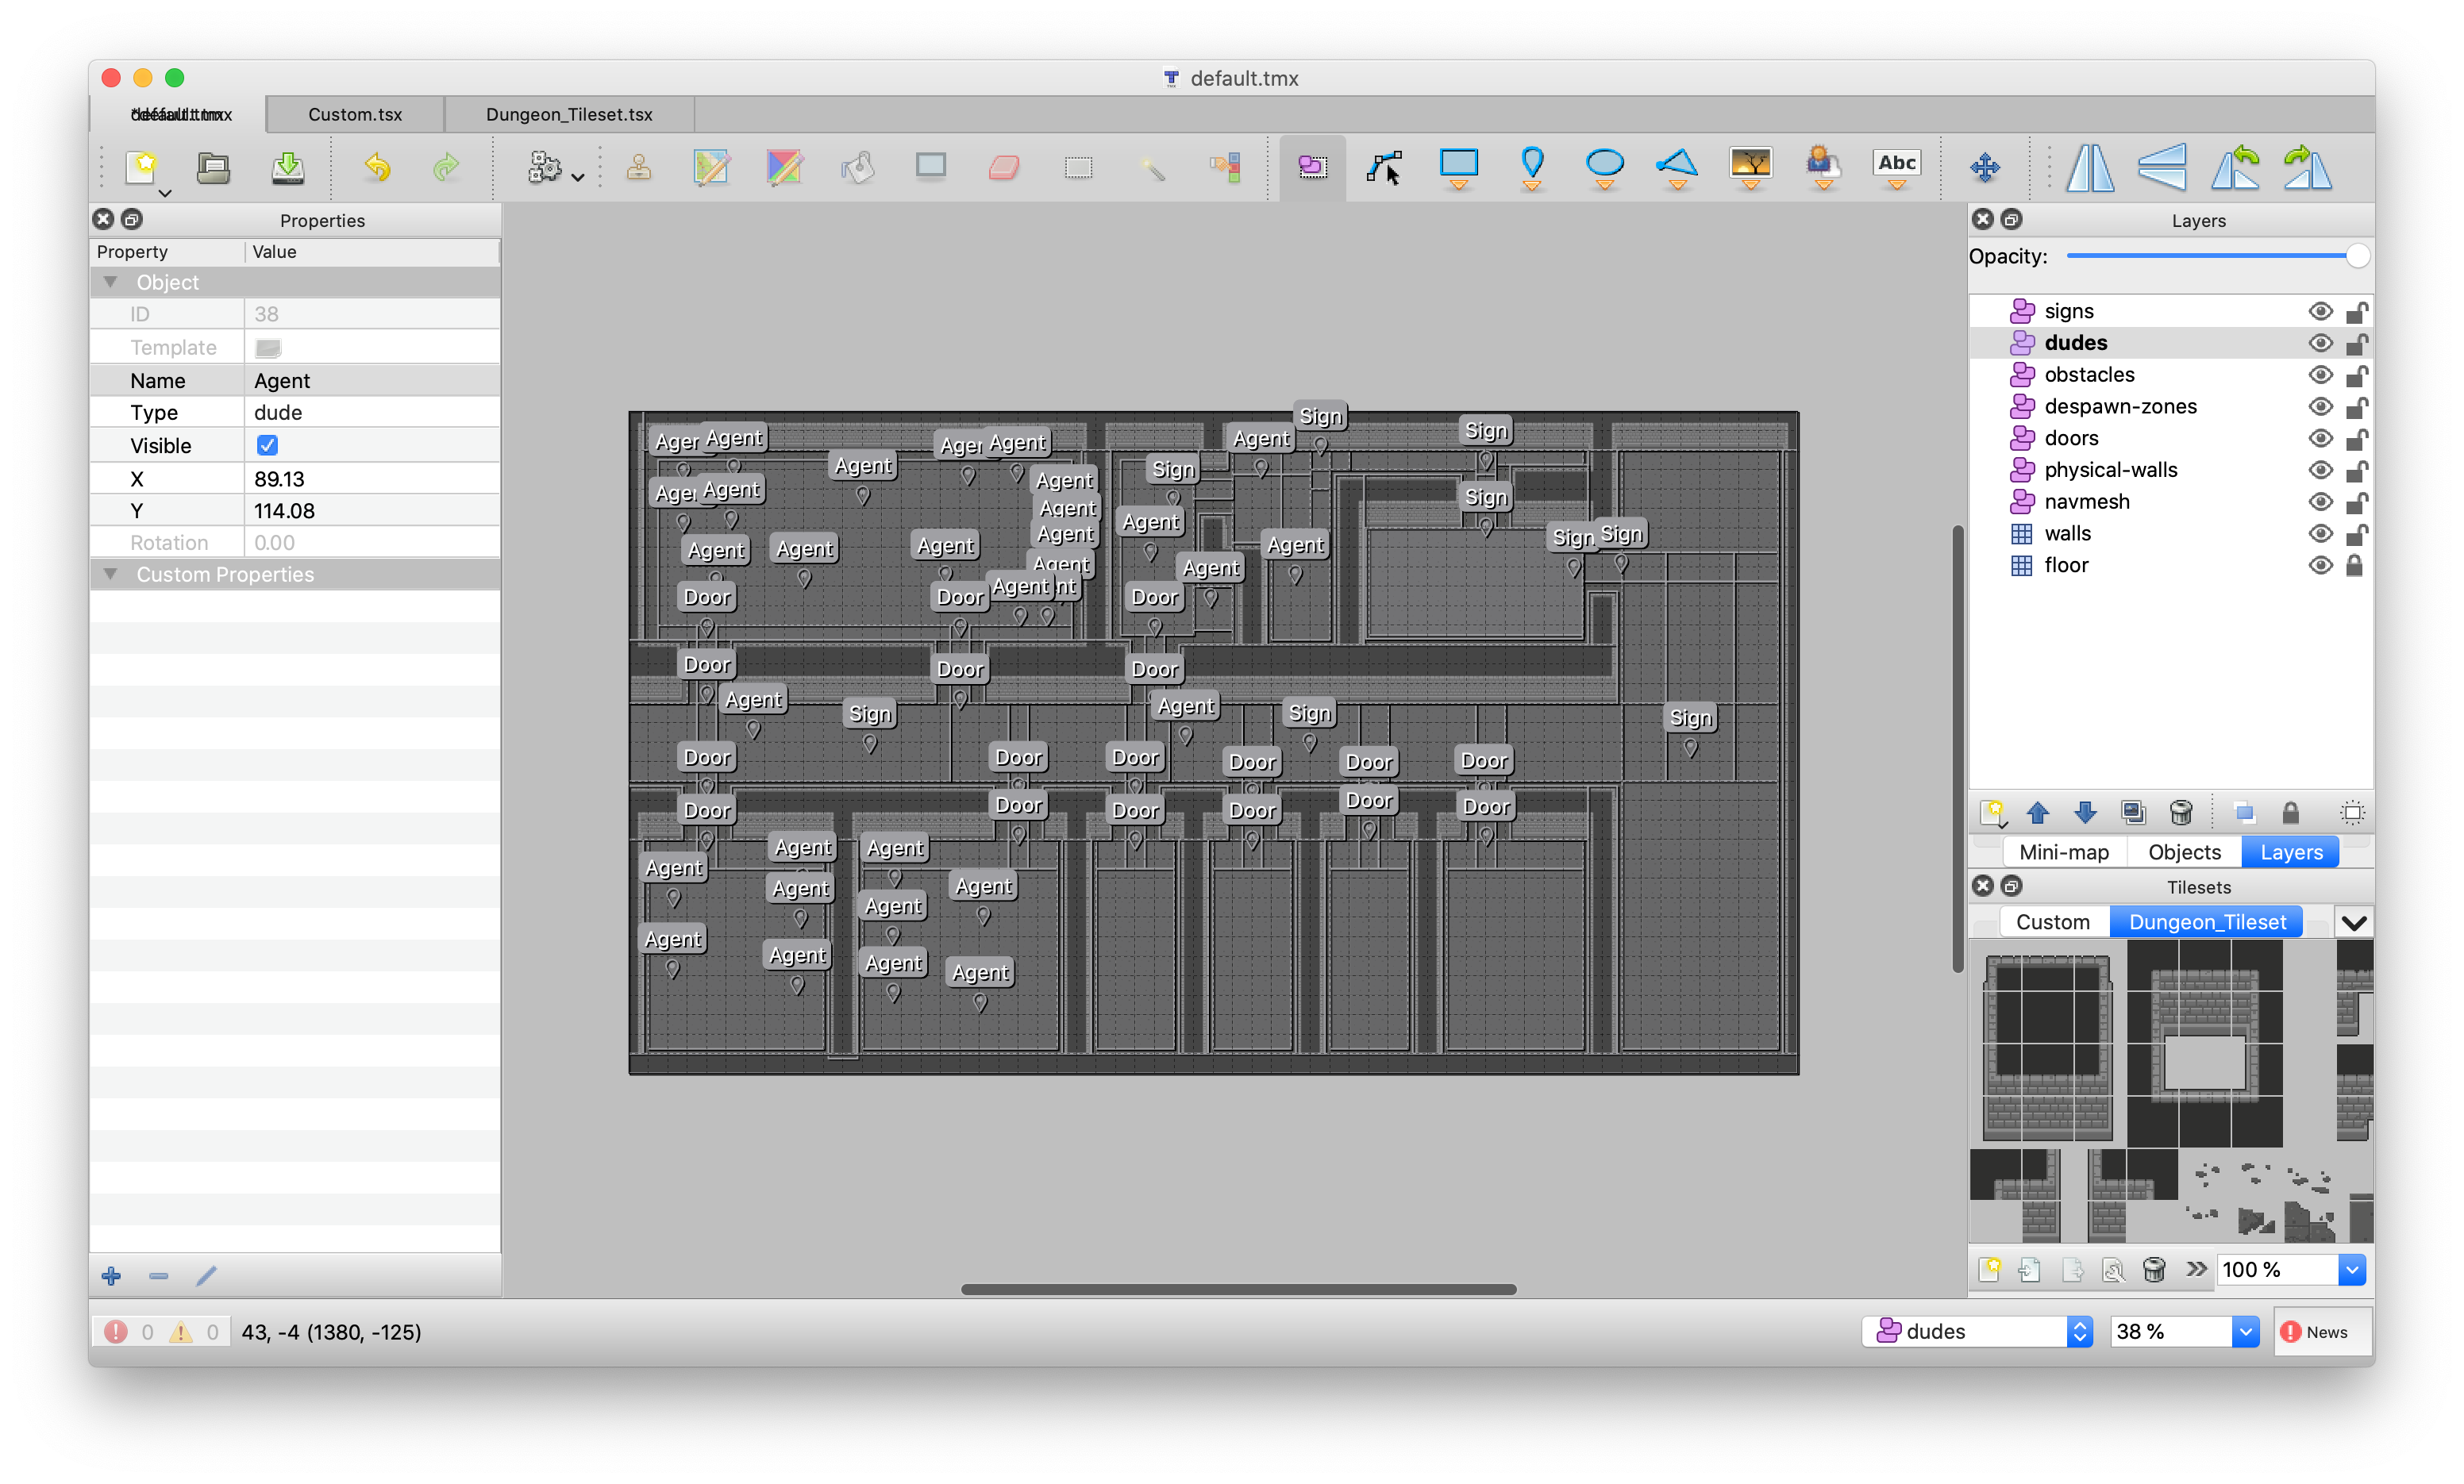
\includegraphics[width=1\linewidth]{assets/tiled-editor}\\
	The editing screen of Tiled
\end{figure}

Using this editor anyone with basic computer skills is able to adjust the given examples or of course define their own settings enabling people using this model as a basic evaluation method of the safety in a case of fire.

\subsection{Agent behaviour}

As phaser includes a physics engine we can make use of this by simulating the behaviour of the agents based on forces acting on them where the final movement is the vector addition of all these forces. Phaser has an \texttt{update} function that is called every time a new frame is calculated. which is perfectly suited for such a task. The different behavioural rules are implemented as follows

\begin{itemize}
    \item Wall repulsion
    
    -

    \item Agent repulsion
    
    Agent repulsion can be implemented rather easily: for every pair of agents a force
    
    \begin{align*}
    	f_r = c_1 \cdot e^{-\frac{d}{c_2}}
    \end{align*}
    
    where $c_1$ and $c_2$ are adjustable parameters but constant for the two agents and $d$ is the distance between the two agents. As the force is proportional to $e^{-d}$, the force is exponentially decreasing when linearly increasing the distance, i.e. exponentially increasing when linearly decreasing it. The initial values for $c_1$ and $c_2$ were empirically determined and are dependant on phasers units and on the agent attraction force.

    \item Agent attraction
    
    The agent attraction force is, in contrast to the agent repulsion force, linearly dependant on the distance $d$
    
    \begin{align*}
    	f_a = c_3 / d
    \end{align*}
    
    but of course directed in the opposite direction of $f_r$. As $f_r$ is exponentially dependant on $d$ and $f_a$ just linearly there is a distance $d_0$ for which the two forces are in balance and the two agents will stay in place if no other force would act on them.

    \item Target attraction
    
    For checking what signs are visible, we iterate over all of them and use a technique called raytracing. This means we draw a line from the agent's position to the sign's position and check whether this line intersects any rectangle defined in the environments \texttt{physical-walls} layer. 
    
    \begin{figure}[H]
		\centering
		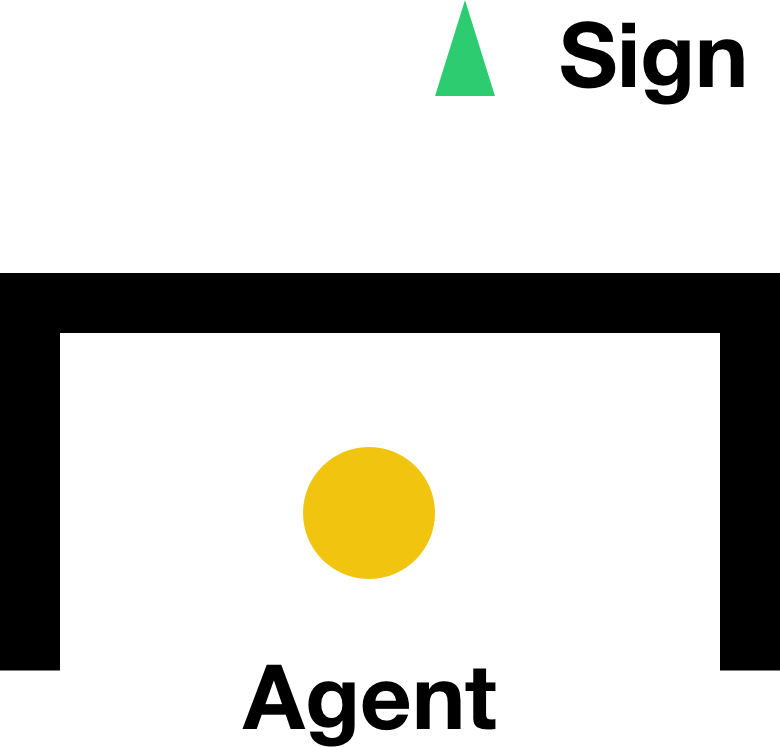
\includegraphics[width=0.25\linewidth]{assets/raytrace-blocked}\\
		An agent's vision blocked by a wall
	\end{figure}
	
	In the figure above the agent is surrounded by walls meaning a line between the agent and the sign would intersect the front wall and thus in this case the agent wouldn't move towards the sign.
	
	\begin{figure}[H]
		\centering
		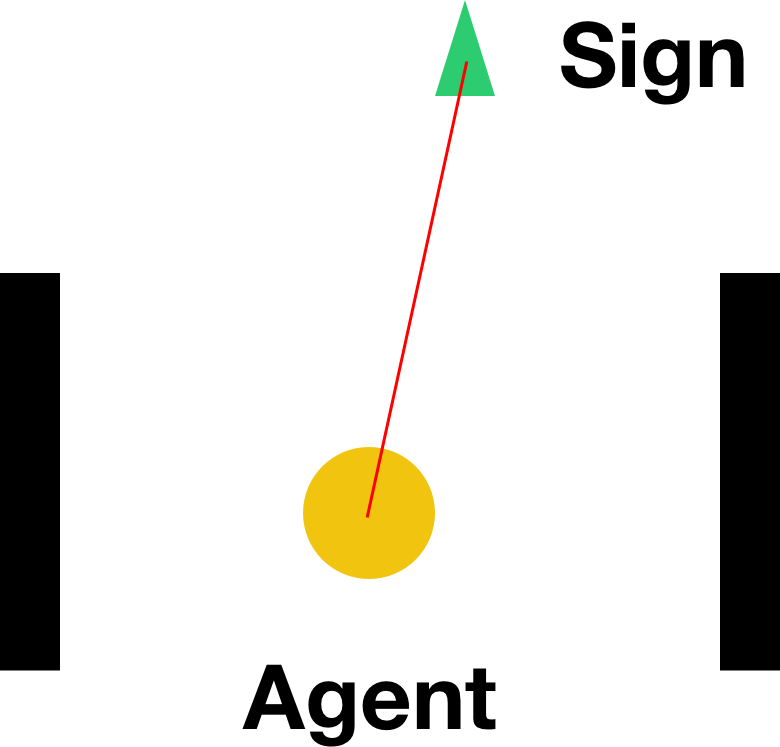
\includegraphics[width=0.25\linewidth]{assets/raytrace-visible}\\
		An agent's sight of a sign visualized by a red ''ray''
	\end{figure}
    
    If that's not the case, the sign is indeed visible and we can apply a force into the direction of the sign. This works fine until you introduce obstacles drawn in gray instead of black which stands for a wall. Obstacles collide with the agent as de walls, meaning the agent won't ''climb'' over it, the difference is that the agent can see ''through'' or over an obstacle. A good example for obstacles are tables.
	
	Now the issue with directly applying a force to the agent into the direction of the ray becomes obvious, the agent will get stuck as it cannot move through the wall. To circumvent this issue, an so called pathfinding algorithm is used, once the agent sees a sign. Now the agent doesn't just move into the targets direction but rather finds a way to the target and this way is able to walk around obstacles. The way this pathfinding algorithm works is by using the \texttt{navmesh} layer in the environment definition that is made up of rectangles which the agent can use as a path. It then creates an ordered list of points that the agent can follow in order to get to the target position.
	
	\begin{minipage}{.4\textwidth}
		\begin{figure}[H]
			\centering
			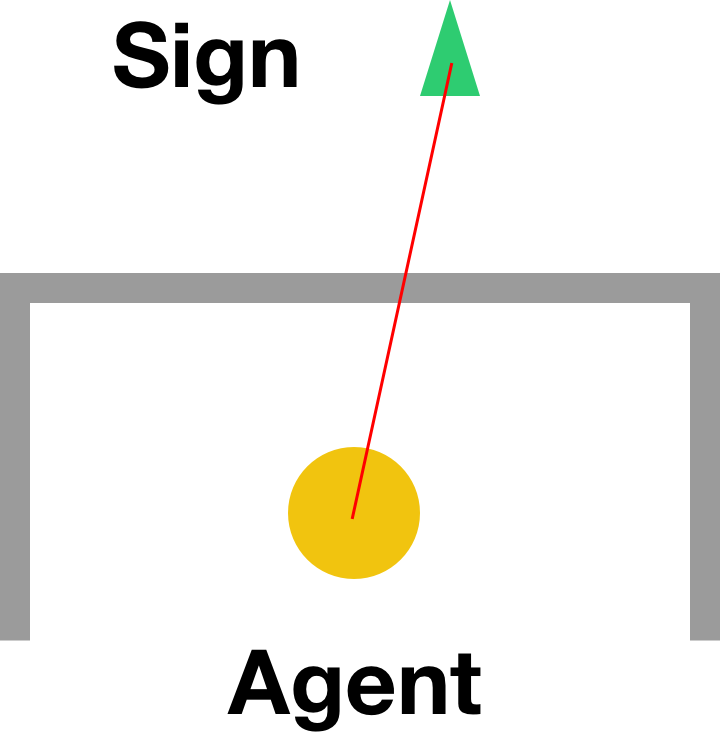
\includegraphics[width=.5\linewidth]{assets/without-navmesh}\\
			Agent stuck within obstacles
		\end{figure}
	\end{minipage}
	\begin{minipage}{.2\textwidth}	
	\vfill\hfill
	\end{minipage}
	\begin{minipage}{.4\textwidth}
		\begin{figure}[H]
			\centering
			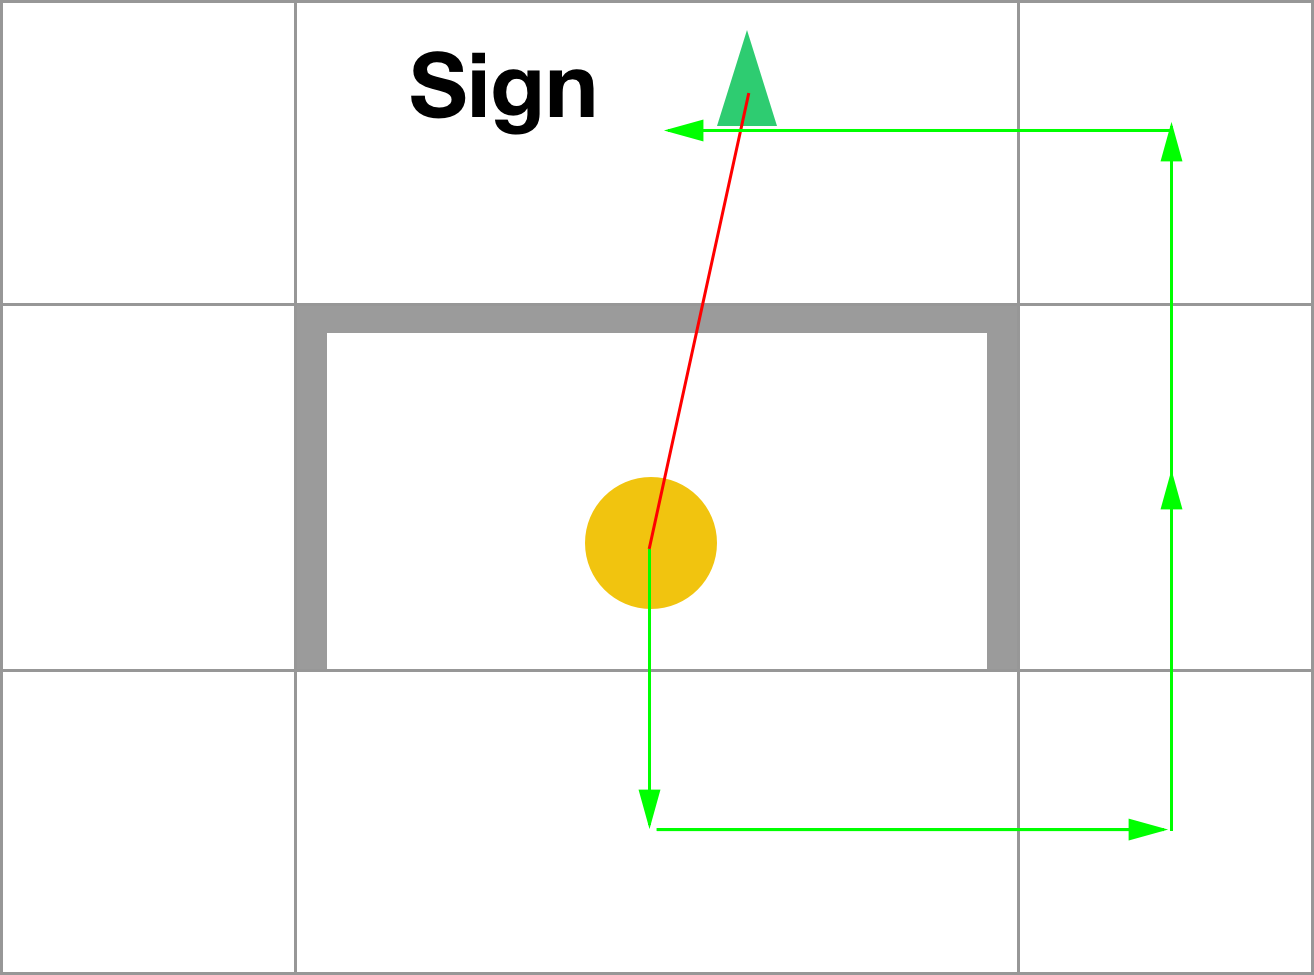
\includegraphics[width=1\linewidth]{assets/with-navmesh}\\
			Agent boxed in obstacles using pathfinding
		\end{figure}
	\end{minipage}
    
\end{itemize}
As soon as we know the target of an agent, we can compute the velocity-correcting force, which tries to accelerate the current physical velocity $v^0$ of the agent to the desired velocity $v$. We compute the force by    
\begin{align*}
  f_t = m*\frac{v^0-v}{\tau}
\end{align*}
where $m$ and $\tau$ are constants, that can be interpreted as the mass and the reactiontime of an agent.

\section{Simulation Results and Discussion}
To test our tool againts existing papers, we tried to replicate experiments of an existing article \cite{Helbing}. Our experiment 1 was described in \cite{Helbing}, whereas our experiment 2 was shown in the video that belongs to the article \cite{Helbing}.  

Some Ideas for experiments: One door for example 100 dudes. Vary the desired velocity and observe how long it takes until all have passed the door.
With obstactle in front of the door versus without, observe how long it takes.


\subsection{Experiment 1}

For the first experiment we replicated the experiments from the paper \cite{Simulating dynamical features of escape panic} from Dirk Helbing, Illés Farkas and Tamás Vicsek in which the agents had to pass a bottleneck in an escape situation. The conclusion was there is an optimal velocty of about $1.5 m/s^-1$ at which all 200 agnets left in the least amount of time. For our model this simulation was quite difficulte to reproduce since our model was highly sensitive towards the friction parameter. This lead to a situation where the agents arranged themselves around the bottleneck in a stable compositon with no progress. This is not representative for a real world escape situation, since humans still react enough reasonable and intelligent under stress to avoid a permanent jam. Therefore all of our statistics were not representative in order to verify this experiment.  

\subsection{Experiment 2}

\subsection{Experiment 3}

\subsection{Interpretation of the simulation result}
When running the simulation several times with a range of different parameters, we can observe some similar behaviour as it is already described in other articles.

\subsubsection{Clogging}
When running the simulation, one might notice that the agents competing for a door are closer together. This is due to the fact, that all agents are pushing towards the door, and hence pushing them together. It worsens the situation, as the friction between the agents increases, which slows down the escape.  
    
\subsubsection{Keeping the distance}
Interestingly, we can observe how agents are pushed back into rooms. Sometimes one could even witness how some agents use another path to avoid the crowd. This is actually what we would expect because of the mutual repulsion of the agents. 

\subsubsection{'Faster-is-Slower effect'}
There are already many published papers regarding the social-force-model. Of which many describe the 'Faster-is-Slower effect' \cite{Helbing, Wang}. The 'Faster-is-Slower effect' describes the phenomenon where the escape through an exit door is slower if the agents are pushing harder. When running our simulation on our default map, we did not observe this effect. The chances are, that this is due to the long corridor, where the agents make up time with a higher speed.

\subsection{Adapting the parameters for better results}

\subsection{Finding the model's limits}


\subsubsection{Evaluation of the building model}
\subsubsection{Evaluation of the agent model}
%The target attraction probably could have been modeled in a better way, instead of simply applying a force into the direction of the target, a real pathfinding algorithm could try to find the fastest way to the target that may involve walking around obstacles. In the current implementation agents fail to walk to the target if they are boxed in into the direction of the target.

\subsection{Evaluation of the simulation}

\section{Summary and Outlook}
- agents should only interact via forces if they can see each other (improve using raytracing)
- use empirical values for the parameters and constants
- use a more stable physics engine
- implement a random fluctuating force to prevent deadlocks

%\section{References}

%To add references, search the paper on https://www.researchgate.net/publication/12295370_Simulating_Dynamic_Features_of_Escape_Panic/citation/download
% and then copy the BibTeX Citation into the file refs.bib

\bibliographystyle{plain}
\bibliography{refs}

\end{document}  



 
